\documentclass[12pt,letterpaper]{article}
\usepackage{fullpage}
\usepackage[top=2cm, bottom=4.5cm, left=2.5cm, right=2.5cm]{geometry}
\usepackage{amsmath,amsthm,amsfonts,amssymb,amscd}
\usepackage{lastpage}
\usepackage{enumerate}
\usepackage{fancyhdr}
\usepackage{mathrsfs}
\usepackage{xcolor}
\usepackage{graphicx}
\usepackage{listings}
\usepackage{hyperref}
\usepackage{multicol}

\usepackage{enumitem}


\hypersetup{%
  colorlinks=true,
  linkcolor=blue,
  urlcolor=cyan,
  linkbordercolor={0 0 1}
}
 
\renewcommand\lstlistingname{Algorithm}
\renewcommand\lstlistlistingname{Algorithms}
\def\lstlistingautorefname{Alg.}

\lstdefinestyle{Python}{
    language        = Python,
    frame           = lines, 
    basicstyle      = \footnotesize,
    keywordstyle    = \color{blue},
    stringstyle     = \color{green},
    commentstyle    = \color{red}\ttfamily
}

\setlength{\parindent}{0.0in}
\setlength{\parskip}{0.05in}

% Edit these as appropriate
\newcommand\course{PHYS 243}
\newcommand\hwnumber{3}                  % <-- homework number
\newcommand\MyName{TA: Abtin Shahidi}           % <-- My name

\pagestyle{fancyplain}
\headheight 35pt
\lhead{\MyName}

\chead{\textbf{\Large Final project}}
\rhead{\course \\ Deadline:  06/15/2019, 11:59 pm}
\lfoot{}
\cfoot{}
\rfoot{\small\thepage}
\headsep 1.5em

\begin{document}
\section*{Neural Networks:}
As you saw in the lectures and notebook, neural nets are quite effective in classification if you build a reasonable network, and here you are going to build a neural network model for a very simple classification task on the data provided \href{https://abtinshahidi.github.io/files/train_set.txt}{here}. (Use any library you want but explain any method you use from them)

\subsection*{Find the simplest neural networks}
Use different \textbf{activations}, \textbf{number of layers}, \textbf{number of neurons at each layer}, compare their performance and find the simplest neural net. There could be couple of networks that are fairly close in terms of the performance choose anyone you think has the least complexity and explain your reasoning.



\begin{figure}[b!]
\centering
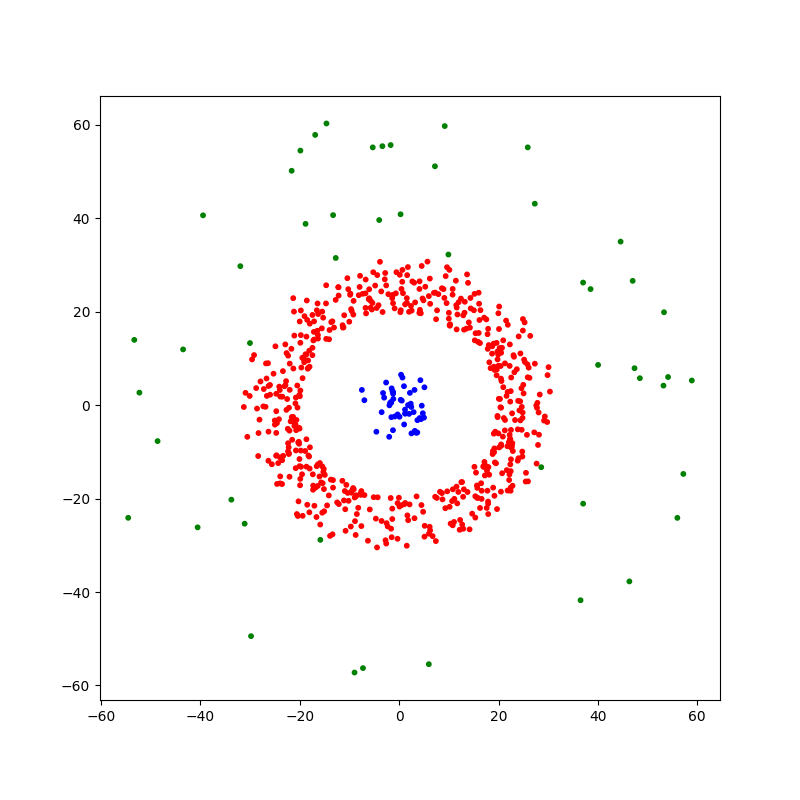
\includegraphics[scale=0.5]{data.png}
\caption{This is how the dataset look like}
\end{figure}



\subsection*{Build new attributes}
In this section you will create new attributes and you are going to use them instead to train the neural network. If we call the first attributes $X_1$ and the second attributes $X_2$, we can build new attributes.

\begin{align*}
X_3 &= X_1^2 \\ 
X_4 &= X_2^2 \\
X_5 &= X_1 X_2
\end{align*} 

Find the simplest Neural network for the following set of inputs: (The data that you feed into the neural network.

\begin{enumerate}
\item $\{X3, X4\}$
\item $\{X3, X5\}$
\item $\{X3, X4, X5\}$
\item $\{X1, X2, X3, X4, X5\}$
\end{enumerate}


\textbf{The data provided to you is the training set and I will check your models again the test set. So remember to evaluate your models and avoid overfitting.} 


\end{document}


